\chapter[狭义相对论]{\itr{Special relativity}{狭义相对论}}
\begin{solution}[{\large\color{plainred}Fizeau effect}\\In this problem we show that the relativistic velocity addition law can be used to
	explain the Fizeau experiment without invoking the existence of \itr{ether}{以太}. The speed of light in stationary water is less than its speed $c$ in \itr{vacuum}{真空}.
	Traditionally it is written as $\frac{c}{n}$, where $n\approx \frac{4}{3}$ is the \itr{index of refraction}{折射率} of water. The water flowed in the \itr{pipe}{管道} with
	velocity $v$. In the lower arm $T_2$ of the \itr{interferometer}{干涉仪} (as shown in the figure), one would expect that, from the nonrelativistic addition law, the
	speed of light in the moving water would be its speed in stationary
	water increased by the speed of the water in the pipe $w=\frac{c}{n}+v$. Show
	that the relativistic velocity addition law leads to, up to higher-order
	corrections:
	\begin{equation*}
		w=\frac cn+v\left(1-\frac1{n^2}\right)
	\end{equation*}
	The result was observed by Fizeau in 1851, but for long time viewed as
	a confirmation of a rather \itr{elaborate}{复杂的} \itr{contemporary}{同时代的} ether-theoretical
	calculation based on the idea that the water was partially successful in
	dragging ether along with it. Einstein later said that it was of
	fundamental importance in his thinking.]
      \begin{center}
      	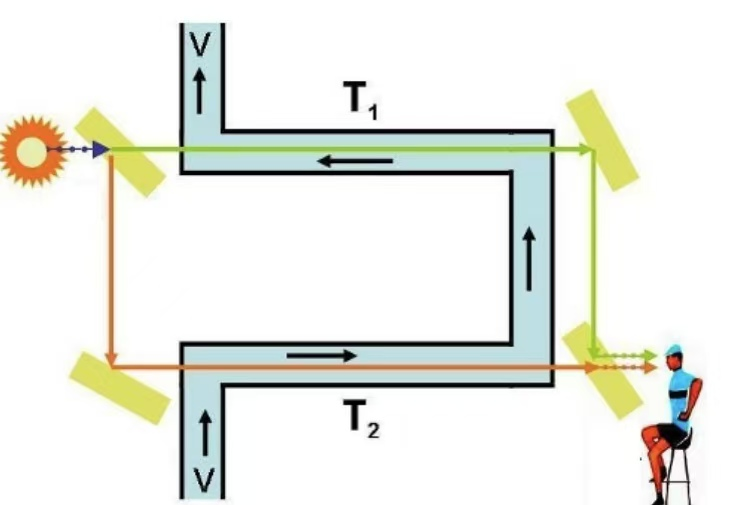
\includegraphics[width=5.5cm, height=4cm]{chapter_6_7}
      \end{center}
      此类题目主要是要选取恰当的参考系,并列出对应参数。
      
      以地面为$S$系,水流为$S^{\prime}$系,并设光前进方向为$x$轴正方向。
      
      在$S$系中,静止的水中光速为$\dfrac{c}{n}$,下方水的速度即$S^{\prime}$系相对$S$系的速度为$v$
      
      那么在$S^{\prime}$系中,由速度变换
      
      \[w=\dfrac{\dfrac{c}{n}+v}{1+\dfrac{cv}{nc^{2}}}=\dfrac{\dfrac{c}{n}+v}{1+\dfrac{v}{nc}}\]
      
      注意到$v\ll c$,故$\dfrac{v}{nc}$为小量,利用泰勒展开至一阶:
      \begin{equation*}
      	\dfrac{1}{1+\dfrac{v}{nc}} = 1 - \dfrac{v}{nc} + o\left(v^{2}\right) 
      \end{equation*}
      代入表达式中,并忽略$v^{2}$相关的高阶小量,即有:
      \[w\approx(\frac{c}{n}+v)(1-\frac{v}{nc})=\frac{c}{n}+v(1-\frac{1}{n^{2}})\]
\end{solution}
\begin{solution}[{\large\itr{Terrel Rotation}{特雷尔旋转}}\\  A square with proper-length-$L$ sides flies past you at a speed $v$, in a direction parallel to two of its sides. You stand in the plane of the square. When you see the square at its nearest point to you, show that it looks to you like it is rotated, instead of contracted. (Assume that $L$ is small compared with the distance between you and the square.)]
    \itr{Terrel Rotation}{特雷尔旋转} 是相对论效应之一,即当物体以接近光速运动时,观察者会看到物体在视觉上旋转。
    
    \ctikzfig{chapter6_solution_6_2_2}
    首先,正如图中标明的,由于尺缩效应,与运动同向的边$AB,CD$在$O$系中长度缩短为$sL$。
    
    之后,注意到我们处理的是视觉效应,那么我们就要考虑光信号到达人眼中才能成像的问题。举边$AD$为例,边上的每一个点发出的光到达人眼的时间都是不同的。在这里,我们考虑$A,D$两点。
    
    连接$AO,DO$,由于题目条件中说,人与正方形的距离远远大于$L$,可以认为$D,A,O$\\[1ex]
    近似成一条直线。因此,$A$发出的光比$D$发出的光提前$\dfrac{L}{c}$的时间到达人眼。\\[1ex]
    换而言之,人眼中接受的光信号,其实是某个时刻的$A$发出的信号,以及该时刻前\\[1ex]
    $\dfrac{L}{c}$的时刻时$D$发出的信号。人眼同时处理这两个信号,产生了“观察到$DA$边”的\\[1ex]
    效果。
    
    \ctikzfig{chapter6_solution_6_2_3}
    
    这张图中的$D_v-A_v-B_v$显示了人眼中观察到的现象。$A_vB_v$的长度即由于尺缩效\\[1ex]
    应得到的$sL$,而$A_vD_v$的长度则等于光信号时间差$\dfrac{L}{c}$乘以正方形运动的速度$v$,也\\[1ex]
    即$\beta L$。
    
    这里我们发现,恰有$(\beta L)^2 + (sL)^2 = L^2$。因此,人眼所看见的,就好像是图中旋转后的正方形$ABCD$在运动方向的投影。且对于旋转的角度$\theta$,有
    \[\sin\theta=\dfrac{\beta L}{L}=\beta\]
\end{solution}
\begin{solution}[{\large\color{plainred}Lots of transformations}\\A train with proper length $L$ moves at speed $\dfrac{c}{2}$ with respect to the ground. A ball is thrown from the back to the front, at speed $\dfrac{c}{3}$ with respect to the train. How much time does this take, and what distance does the ball cover, in:
	\\(a) The train frame?
	\\(b)The ground frame? Solve this by:
	\\\hspace*{2em}i. Using a velocity-addition argument.
	\\\hspace*{2em}ii. Using the Lorentz transformations to go from the train
	frame to the ground frame.
	\\(c)The ball frame?
	\\(d) Verify that the \itr{invariant interval}{不变(时空)间隔} is indeed the same in all three
	frames.]
         \begin{singlefigure}{chapter_6_19}[0.6]        
        \end{singlefigure}
        (a)火车相对自身是静止的,故火车系下其长度就是原长,而火车系下球的速度已知,故有
        \begin{equation*}
        	\begin{aligned}
        		&\Delta x_{1}=L\\
        		&\Delta t_{1}=\frac{L}{c/3}=\frac{3L}{c} \\
        	\end{aligned}
        \end{equation*}
        (b)选取地面为$S$系,火车为$S^{\prime}$系,火车前进方向为$x$正方向。$S^{\prime}$系相对$S$系的速度$u$为
        \[u=\dfrac{c}{2}\]
        (i)$S^{\prime}$系中球的速度为$v^{\prime}=\dfrac{c}{3}$,由速度变换公式有$S$系中,球的速度
        \[v=\dfrac{v^{\prime}+u}{1+\dfrac{{v}^{\prime}u}{c^2}}=\frac{5c}{7}\]
        列车在地面看来会发生尺缩效应,且尺缩因子$s = \sqrt{1-\left(\dfrac{u}{c}\right)^{2}} = \dfrac{\sqrt{3}}{2}$,得地面系中列车长度
        \[ d=sL = \dfrac{\sqrt{3}}{2}L\]
        在$S$系中是一个追及问题,所需时间:
        \[\Delta t_2=\frac{d}{v-u}=\frac{7\sqrt{3}L}{3c}\]
        所走距离
        \[\Delta x_2=vt_{2}=\frac{5\sqrt{3}L}{3}\]
        (ii)利用洛伦兹变换的变化量形式:
        \begin{equation*}
        	\begin{aligned}
        		&\Delta t_2 = \gamma(\Delta t_1 + \frac{u} {c^{2}}\Delta x_1)\\
        		&\Delta x_2 = \gamma(\Delta x_1 + u\Delta t_1)
        	\end{aligned}
        \end{equation*}
        可求得
        \begin{equation*}
        	\begin{aligned}
        		&\Delta t_2=\frac{7\sqrt{3}L}{3c}\\[1ex]
        		&\Delta x_2=\frac{5\sqrt{3}L}{3}\\
        	\end{aligned}
        \end{equation*}
        
        (c)在设球参考系为$S^{\prime \prime}$系,显然$S^{\prime \prime}$系下球是静止的:
        \begin{equation*}
        	\Delta x_3=0
        \end{equation*}   
        $S^{\prime \prime}$系相对$S^{\prime}$系速度$u^{\prime} = \dfrac{c}{3}$,
        有$\gamma^{\prime} = \dfrac{1}{\sqrt{1-\left(\dfrac{u^{\prime}}{c}\right)^{2}}} = \dfrac{3\sqrt{2}}{4}$,利用洛伦兹变换得
        \begin{equation*}
        	\Delta t_{3}= \gamma^{\prime}(\Delta t_1 - \frac{u^{\prime}\Delta x_1} {c^{2}})
        	=\frac{2\sqrt{2}L}{c}
        \end{equation*}
        
        (d)题意其实就是要证明时空间隔$(c\Delta t)^2-(\Delta x)^2$的不变性,将之前所求代入验证即可:
        \begin{equation*}
        	\begin{aligned}
        		(c\Delta t_{1})^{2}-(\Delta x_{1})^{2}&=8L^{2} \\
        		(c\Delta t_{2})^{2}-(\Delta x_{2})^{2}&=8L^{2}\\
        		(c\Delta t_{3})^{2}-(\Delta x_{3})^{2}&=8L^{2} \\
        	\end{aligned}
        \end{equation*}
        可见事件的时空间隔确实不变。
        
        注:如果老师上课时定义的时空间隔与此处不同,注意符号问题或者在回答时说明好。
\end{solution}
\begin{solution}[{\large\color{plainred}Train And \itr{Tunnel}{隧道} \itr{Paradox}{悖论}}\\
	Consider a train running at a constant speed $V$ on the straight track in the $x$ direction, and passing through a tunnel (see the figure). The proper length of the train is $L$, and the proper length of the tunnel is $D$. Here we assume $L>D$. Define $(x,ct)$ as the time and the space coordinates of the track frame, and $(x',ct')$ as those of the train frame. Here, $x$ and $x' $\textbf{ are in the same direction}.	
	\\
	(a) Suppose that an observer standing on the ground sees that the train is shorter than the tunnel, so that the whole train can be inside the tunnel. Determine the smallest possible speed of the train.
	\\
	(b) Suppose that the rear end of the tunnel (see the figure) is at $x=0$, and set the time $t=t'=0$ when the rear end of the train reaches the rear end of the tunnel. Draw the Minkowski diagram \textbf{ taking $x$ coordinate for the horizontal axis and $ct$ coordinate for the vertical axis.} In addition, \itr{specify}{指明} $L$ and $D$ in the diagram.
	\\
	(c) When the rear end of the train enters the rear end of the tunnel, the rear-end and front-end sliding doors of the tunnel (see the figure) are closed at the same time in the track frame. These two events are denoted by $R_{close}$ and $F_{close}$, respectevely. Then, when the front-end of the train reaches the front end of the tunnel, both the rear-end and front-end sliding doors are opened at the same time in the track frame. These events are denoted by $R_{open}$ and $F_{open}$, respectively.
	\\
	Show the events $R_{close},F_{close},R_{open}$, and $F_{open}$ in the Minkowski diagram in (b),
	and put the four events in the order of being seen by an observer in the train.
	]
	\begin{singlefigure}{chapter_6_20}[1]    
	\end{singlefigure}
    (a)
    \\根据尺缩效应,在轨道参考系中,火车的长度为
    \[\sqrt{1-\dfrac{v^2}{c^2}}L\]
    故如需火车能够完全在隧道中,则有
    \[\sqrt{1-\dfrac{v^2}{c^2}}L\le D\]
    可解得
    \[v\ge \sqrt{1-\dfrac{D^2}{L^2}}c\]
    (b)\\
    作图如下:
    \begin{center}
    	\resizebox{16.2em}{12em}{\tikzfig{chapter6_solution_6_4_1}}
    \end{center}
    
    
    依据题意,隧道尾和火车尾在$0$时刻都处于$O$点。由于隧道在轨道系中静止,隧道在轨道系中的长度即为其原长$D$。因此,在$x$轴上取长度$D$,对应的$P$点即是$0$时刻时隧道头的位置。
    
    首先,需要过$P$做校准曲线,与$x'$轴相交于$Q_1$点。由于题目条件$L>D$,因此$L$的端点在$Q_1$右侧。
    
    另外,还需要过$P$作$ct'$轴的平行线,交$x'$轴于$Q_2$点。这是因为列车在轨道系(也就是$x-ct$系)中的长度应当小于$D$,且列车头的世界线斜率与$ct'$轴斜率相同。于是,过$L$的端点作$ct'$轴的平行线与$x$轴的交点应在$P$的左侧,等价于$L$的端点在$Q_2$的左侧。
    
    综上,任取一点在$Q_1,Q_2$之间,它与$O$的距离就可以表示$L$。
    (c)\\
    根据题意作出图如下
    \begin{singlefigure}{chapter_6_22}[0.6]   
    \end{singlefigure}
    作出平行线后发现
    \[{t_1}^{\prime}<{t_2}^{\prime}<{t_3}^{\prime}<{t_4}^{\prime}\]
    故有
    \[F_{close}\rightarrow F_{open}\rightarrow R_{close}\rightarrow R_{open}\]
\end{solution}
\begin{solution}[{\large\color{plainred}Conservation of momentum in SR}]
      (i)由速度变换 
        \[v^{\prime}=\frac{v+v}{1+\frac{v^{2}}{c^{2}}}=\frac{2v}{1+\frac{v^{2}}{c^{2}}} \]
      (ii)对于红色粒子
        \[v_{xr}=0\]
        \[v_{yr}=\frac{v\sqrt{1-\beta^{2}}}{1+\frac{0v}{c^{2}}}=v\sqrt{1-\frac{v^{2}}{c^{2}}}\] 
        对于蓝色粒子
        \[v_{xb}=v\] 
        \[v_{yb}=\frac{-v\sqrt{1-\beta^{2}}}{1+\frac{0v}{c^{2}}}=-v\sqrt{1-\frac{v^{2}}{c^{2}}} \]
     (iii)在$k^{\prime}$系下\\
         碰前动量
        \[\overrightarrow{P_{0}}=\frac{mv^{\prime}}{\sqrt{1-(\beta^{\prime})^{2}}}\overrightarrow{i},\beta^{\prime}=\frac{v^{\prime}}{c}=\frac{2\beta}{1+\beta^{2}}\]
        代入发现
        \[P_{0}=\frac{2mv}{1-\beta^{2}}\overrightarrow{i}\]
        碰后动量
        \[\overrightarrow{P}=\frac{2mv}{\sqrt{1-(\beta^{\prime\prime})^{2}}}\overrightarrow{i}\]
        注意此时
        \[\beta^{\prime\prime}=\frac{\sqrt{v_x^{2}+v_y^{2}}}{c}\]
        故$\beta^{\prime\prime}=\beta\sqrt{2-\beta^{2}}$\\
        代入后有
        \[\overrightarrow{P}=\frac{2mv}{1-\beta^{2}}\overrightarrow{i}\]
        故$\overrightarrow{P}=\overrightarrow{P_{0}}$,动量守恒

\end{solution}
\begin{solution}[{\large\color{plainred}Perfectly Inelastic Collison of two Relastivistic Particles}]
    (a) 由能量守恒
    \[\frac{mc^2}{\sqrt{1-\frac{v^2}{c^2}}}=Mc^2\]
    故$M=\frac{m}{\sqrt{1-\frac{u^{2}}{c^{2}}}}$
    (b)由速度变换
    \[u=\frac{v+v}{1+\frac{v^{2}}{c^{2}}}=\frac{2v}{1+\frac{v^{2}}{c^{2}}}\]
    (c)碰前动量
    \[P_{0}=\frac{mu}{\sqrt{1-\frac{u^{2}}{c^{2}}}}=\frac{2mu}{1-\frac{v^{2}}{r^{2}}}\]
    碰后动量
    \[P=\frac{2Mv}{\sqrt{1-\frac{v^{2}}{c^{2}}}}=\frac{2mv}{1-\frac{v^{2}}{c^{2}}}\] 
    $P=P_0$,故动量守恒\\
    碰前能量 
    \[E_{0}=mc^{2}+\frac{mc^{2}}{\sqrt{1-\frac{u^{2}}{c^{2}}}}=\frac{2mc^{2}}{1-\beta^{2}}\]
    碰后能量
    \[E=2\frac{Mc^{2}}{\sqrt{1-\frac{v^{2}}{c^{2}}}}=\frac{2mc^{2}}{1-\beta^{2}}\]
    $E=E_0$,故能量守恒。
\end{solution}
\begin{solution}[{\large\color{plainred}Relastivistic Scattering between a Photon and an Electron}]
(a)\\   
    (i)\[E=\frac{mc^{2}}{\sqrt{1-\frac{1}{t^{2}}}},\mathbf{P}=\frac{m\mathbf{v}}{\sqrt{1-\frac{v^2}{c^{2}}}}\]
    (ii)由速度变换
    \[v^{\prime}=\frac{v-u}{1-\frac{uv}{c^2}}=\frac{\beta_{v}-\beta_{u}}{1-\beta_{u}\beta_{v}}\]
    又$\gamma^{\prime}=\frac{1}{\sqrt{1-\frac{{v^{\prime}}^{2}}{c^{2}}}}$
    故有
    \[\frac{1}{{\gamma^{\prime}}^{2}}=\frac{1}{\gamma^{2}}\frac{1}{\gamma_{u}^{2}}(1-\beta_{u}\beta_{v})^{2}\]
    即$\gamma^{\prime}=\frac{\gamma_{u}\gamma}{1-\beta_{u}\beta_{v}}$
    故$\frac{E^{\prime}}{c}=\gamma^{\prime}\frac{mc^{2}}{c}=(\frac{E}{c}-\frac{|\mathbf{P|}u}{c})\gamma_{u}$
    \[\mathbf{P^{\prime}}|=(|\mathbf{P}|-\frac{uE}{c^{2}})\gamma_{u}\]
(b)\\
(i) \[\mathbf {P}\cdot \mathbf{P}= \frac {E^{2}}{c^{2}}- P^{2}\]
又$E^2-p^2c^2=m^2c^4$ \\
故$\mathbf{P}\cdot\mathbf{P}=m^2c^2$\\
 (ii) 
\[{\mathbf{P}} ^{\prime }\cdot {\mathbf{P}} ^{\prime }= \frac {{E^{\prime}}^2-{p^{\prime}}^{2}c^{2}}{c^{2}}= m^{2}c^{2}= \mathbf{P} \cdot \mathbf{P}\]
(iii)\\
\[\mathbf{k}\cdot\mathbf{k}=0\]
(c)\\
换到以$u$运动系中,\\
入射前
\[\vec{P}(p,p,0,0),\vec{P}_{e}(mc,0,0,0)\]
入射后
\[\vec{P}^{\prime}(p^{\prime},-p^{\prime},0,0),\vec{P_e}^{\prime}(b_{mc},\delta_{m}v,0,0)\]
\[\vec{P}+\vec{P}_{e}=\vec{P}_{e^{\prime}}+\vec{P}^{\prime}\]
即\[\vec{P}-\vec{P}^{\prime}=\vec{P_e}^{\prime}-\vec{P_e}\]
取平方
\[\vec{P}^2+{\vec{P}^{\prime}}^2-2\vec{P}^2{\vec{P}^{\prime}}^2={\vec{P_e}^{\prime}}^2+\vec{P_e}^{2}\]
并注意到
\[\vec{P^{2}}={\vec{P^{\prime}}}^{2}=0\]
\[{\vec{{P_e}^{\prime}}}^{2}=\vec{P_e^{2}}=m^{2}c^{2}\]
故\[2\vec{P}\cdot\vec{P^\prime}=(\gamma-1)m^{2}c^{2}\]
\\又能量守恒
\[(\gamma-1)mc^{2}=pc-p^{\prime}c\]
消去$\gamma$,故
\[\frac{1}{P^{\prime}}=\frac{1}{P}+\frac{2}{mc}\]
即\[\frac{1}{E_{Ph}^{\hbar}}=\frac{1}{E_{Ph}}+\frac{1}{mc^{2}}\]
\end{solution}